% Capítulo 3

\chapter{Desenvolvimento da biblioteca mirobot-poti}
\label{cap:descricao}
% breve descrição da estrutura do capítulo
% url do github contendo o projeto

Este capítulo está dividido em quatro seções, as quais simboliza as etapas do
desenvolvimento da biblioteca mirobot-poti. A primeira seção descreve o protocolo de funcionamento
do mirobot e a definição da classe mirobot, assim como os seus métodos. A
segunda seção, apresenta o processo de
implementação da biblioteca e, após o seu desenvolvimento exemplificar com um
caso de uso a usando o potigol. A terceira seção descreve a parte de empacotamento do projeto. A quarta seção finaliza com exemplos de
código e testes da implementação. O código do projeto que foi desenvolvida está disponível em:
\url{https://github.com/ensino-de-programacao/mirobot-potigol}.

\section{Definição dos métodos}
\label{sec:definicao}
% descrição do protocolo de comunicação
% Definição da classe Mirobot e dos seus métodos
O início do desenvolvimento do mirobot-poti se baseou principalmente na
biblioteca mirobot-py
(\url{https://github.com/mirobot/mirobot-py}). O mirobot-py contém
os artifícios necessários para se comunicar com mirobot por meio da linguagem
Python, esse código se baseia em uma classe principal que representa o robô
mirobot e seus métodos (ações).

\begin{figure}[H]
\centering
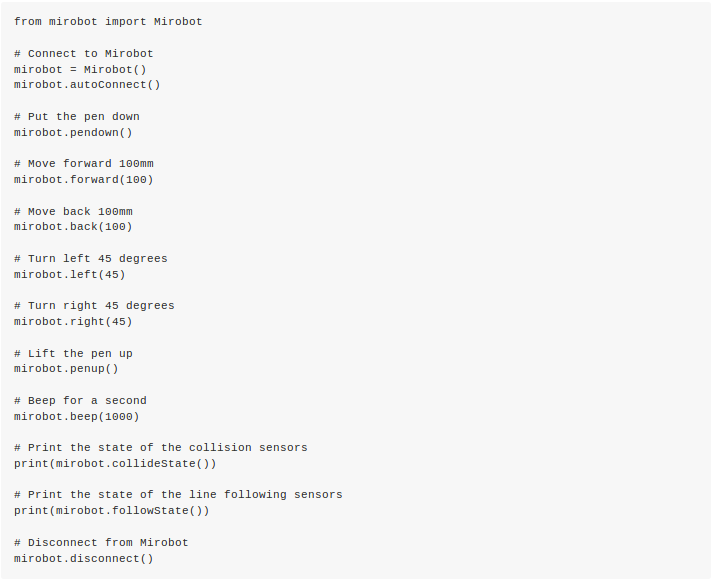
\includegraphics[scale=0.45]{imagens/desc-api.png} 
\label{fig:descapi}
  \textsf{\caption{Definição de alguns métodos da classe principal do
  mirobot-py.}}
\end{figure}

Como pode ser visto na Figura 1, esses são os métodos da classe Mirobot. Dentre eles estão os que têm o propósito de se conectar com o robô: tanto
automaticamente, por meio de uma detecção automática dos dispositivos mirobot;
quanto manualmente, inserindo o endereço IP do robô e a porta de comunicação
desejada; e por último um método para se desconectar e fechar a conexão
WebSocket. Além dos métodos de conexão, ainda tem os de movimentação, e entre
eles estão: a movimentação para trás e para frente (medida em milímetros),
movimentação para os lados (girar sobre o próprio eixo usando o grau como
medida) direito e esquerdo, e a ação ``beep'' que recebe um valor em segundos
da duração do som, por último, descer e levantar a caneta. E para finalizar, os
métodos que são responsáveis por: informar a velocidade em que os pacotes estão
sendo enviados e recebidos via Wi-Fi (ping), retorna as informações captadas
pelo sensor de colisão, retornar as informações captadas pelo sensor de
seguimento de linha.

Baseando-se nessas definições, foi criado a classe Mirobot e seus métodos na
linguagem Java. Para poder seguir o padrão do potigol, os nomes dos métodos
foram traduzidos do inglês para o português. Depois de finalizada a etapa de
definição dos métodos foi passado para a etapa de implementação. 

\section{Implementação dos métodos}
\label{sec:implementacao}
% Descrever a implementação
% Exemplo em potigol

A implementação da biblioteca mirobot-poti, foi feita através da linguagem Java.
Para a comunicação via websocket foi usado o projeto
Glassfish Tyrus(\url{https://tyrus.java.net/}). O critério de escolha pelo
Glassfish Tyrus foi devido a possibilidade de usar um servidor \textit{standalone}, ou
seja, um servidor que roda dentro da própria aplicação, caso contrário seria
necessário um servidor externo para abrigar a aplicação. 

Primeiramente foi estudado o funcionamento da biblioteca tyrus e feito alguns
exemplos simples de comunicação websocket. Depois de entendido a parte básica,
foi seguido o próximo passo de criação de um socket handler. O websocket
handler é o responsável por enviar e receber as mensagens do mirobot, ele
representa o baixo nível de comunicação e está diretamente ligado ao websocket.
As mensagens enviadas e recebidas pelo socket handler são no formato JSON (Java
Object Notation), e seguem a seguinte estrutura:

\begin{figure}[H]
\centering
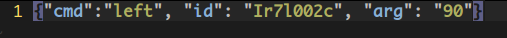
\includegraphics[scale=0.50]{imagens/comandojson.png} 
\label{fig:comandojson}
  \textsf{\caption{Exemplo de comando no formato JSON.}}
\end{figure}

Como pode ser visto na Figura 2, as mensagens JSON que são enviadas do mirobot se
baseiam em três informações: o ``cmd'' que representa o comando desejado que o
mirobot realize; o ``id'' que representa a identificação da mensagem que foi
enviada (posteriormente vai ser explicado a sua utilidade); e o ``arg'' que
representa o argumento que vai ser passado ao comando, se o comando não
precisar de argumento, como é o caso do comando usado para descer a caneta ou
de verificar o ping, esse atributo é ignorado. Então basicamente o
funcionamento da biblioteca em linhas gerais, se resume em traduzir um comando
para o formato JSON e enviá-lo via websocket obedecendo a estrutura
exemplificada na Figura 2. 

O mirobot a cada comando recebido retorna uma mensagem em JSON para informar a
situação da execução do comando recebido. O atributo ``id'' serve para identificar o comando o qual o mirobot está
informando a situação. Outro ponto importante é que, alguns comandos do mirobot
demoram mais para ser executados que outros, dependendo do tamanho do
argumento. Para exemplificar essa questão temos que levar em conta o seguinte
fator, se for enviado um comando para que o mirobot ande 10 mm para frente, ele
irá demorar um certo tempo para poder se deslocar os 10 mm, já se for enviado o
mesmo comando mudando o argumento para 20 mm, o mirobot vai demorar o dobro de
tempo para completar o percurso. 

Considerando que o mirobot não empilha as mensagens recebidas, e executa apenas
uma por vez, fica a cargo da biblioteca fazer esse controle, pois se o robô
receber um comando enquanto estiver no meio da execução de outro, irá ocorrer
um erro. A estratégia usada para resolver esse problema foi a seguinte:
todos os comandos que serão enviados para o mirobot são guardados em uma fila,
e vão sendo enviados à medida que o tempo estimado de duração de um comando
simples seja cumprido, já no caso dos comandos que têm variação de duração em
decorrer do tamanho do argumento passado, usa-se esse mesmo argumento e o
comando enviado para se estimar o tempo que vai ser esperado até o envio do
próximo comando da fila.
 
Depois de completa esses passos, foi incorporado a classe mirobot o \texit{WebsocketHandler}, o qual é usado por todos os seus métodos já
definidos anteriormente. Depois de finalizada essa etapa foi gerado o arquivo
da biblioteca, importado e testado no Potigol.

\section{O Potigol e o empacotamento da biblioteca}
\label{sec:empacotamento}
% Empacontando o projeto

Em paralelo com o desenvolvimento da biblioteca mirobot-poti, foi testado a
importação do formato jar do Potigol, todas as tentativas iniciais foram sem
sucesso pois o Potigol não conseguia fazer a importação do arquivo jar. Depois
de muitas tentativas foi descoberto que o class-path do Potigol não adicionava
os arquivos jar automaticamente, pois apesar de incluso no class-path o
diretório no qual o arquivo jar se encontrava, só era achado dentro do diretório
os arquivos class. O problema foi solucionado descompactando o arquivo jar no diretório
principal do Potigol. Outra forma que daria para resolver esse problema seria adiconando
manualmente o caminho completo do arquivo jar no class-path.

No momento de compilação do projeto mirobot-poti utilizando o maven para
automatizar a compilação, foi usado um plugin do maven chamado
``jar-with-dependences'' para que na hora da compilação as dependências do
projeto (Glassfish Tyrus) seja inserido dentro do arquivo jar, possibilitando
que o projeto após compilado dependa apenas de um único arquivo jar para ser
executado.

\section{Teste da implementação com exemplo de código}
\label{sec:testemirobot}

A última etapa do trabalho ficou com o teste na linguagem Potigol usando a
biblioteca mirobot-poti para se comunicar com o simulador do robô
(mirobot-sim). O para a realização do teste foi usado uma adaptação na classe
mirobot, pois não foi encontrado uma forma de instanciar um novo objeto dentro
do Potigol. Essa adaptação foi o uso do padrão singleton para, a qual a classe
fica responsável por gerar uma instancia da classe e retornar a variável no
Potigol. Após a implementação do teste, foi completa a etapa de desenvolvimento
do trabalho.

\begin{figure}[H]
\centering
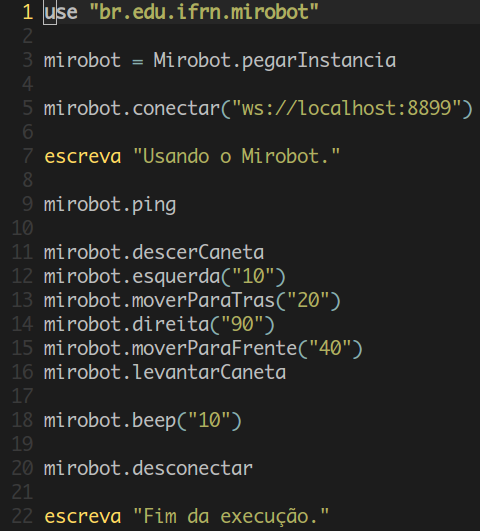
\includegraphics[scale=0.50]{imagens/teste-potigol.png} 
\label{fig:testepotigol}
\end{figure}
